\documentclass[ignorenonframetext,]{beamer}
\usetheme{Warsaw}
\usefonttheme{serif}
\usepackage{amssymb,amsmath}
\usepackage{ifxetex,ifluatex}
\usepackage{fixltx2e} % provides \textsubscript
\usepackage{lmodern}
\ifxetex
  \usepackage{fontspec,xltxtra,xunicode}
  \defaultfontfeatures{Mapping=tex-text,Scale=MatchLowercase}
  \newcommand{\euro}{€}
\else
  \ifluatex
    \usepackage{fontspec}
    \defaultfontfeatures{Mapping=tex-text,Scale=MatchLowercase}
    \newcommand{\euro}{€}
  \else
    \usepackage[T1]{fontenc}
    \usepackage[utf8]{inputenc}
      \fi
\fi
\IfFileExists{upquote.sty}{\usepackage{upquote}}{}
% use microtype if available
\IfFileExists{microtype.sty}{\usepackage{microtype}}{}
\usepackage{letltxmacro}
\makeatletter
\def\maxwidth{\ifdim\Gin@nat@width>\linewidth\linewidth\else\Gin@nat@width\fi}
\def\maxheight{\ifdim\Gin@nat@height>\textheight0.8\textheight\else\Gin@nat@height\fi}
\makeatother
\AtBeginDocument{
  \LetLtxMacro\Oldincludegraphics\includegraphics
  \renewcommand{\includegraphics}[2][]{%
    \Oldincludegraphics[#1,width=\maxwidth,height=\maxheight,keepaspectratio]{#2}}
}

% Comment these out if you don't want a slide with just the
% part/section/subsection/subsubsection title:
\AtBeginPart{
  \let\insertpartnumber\relax
  \let\partname\relax
  \frame{\partpage}
}
\AtBeginSection{
  \let\insertsectionnumber\relax
  \let\sectionname\relax
  \frame{\sectionpage}
}
\AtBeginSubsection{
  \let\insertsubsectionnumber\relax
  \let\subsectionname\relax
  \frame{\subsectionpage}
}

\setlength{\parindent}{0pt}
\setlength{\parskip}{6pt plus 2pt minus 1pt}
\setlength{\emergencystretch}{3em}  % prevent overfull lines
\setcounter{secnumdepth}{0}

\title{Why do Nigerian Scammers Say They are from Nigeria?}
\subtitle{Mineria de Datos - ITAM}
\author{Carlos Petricioli, Liliana Millán, Amanda Balderas}
\date{December 3, 2014}

\begin{document}
\frame{\titlepage}

\begin{frame}{Introducción}

Nos referimos al artículo:

\begin{block}{Why do Nigerian Scammers Say They are from Nigeria?}

Cormac Herley

\emph{Microsoft Researh}

\end{block}

\end{frame}

\begin{frame}{Why do Nigerian Scammers Say They are from Nigeria?}

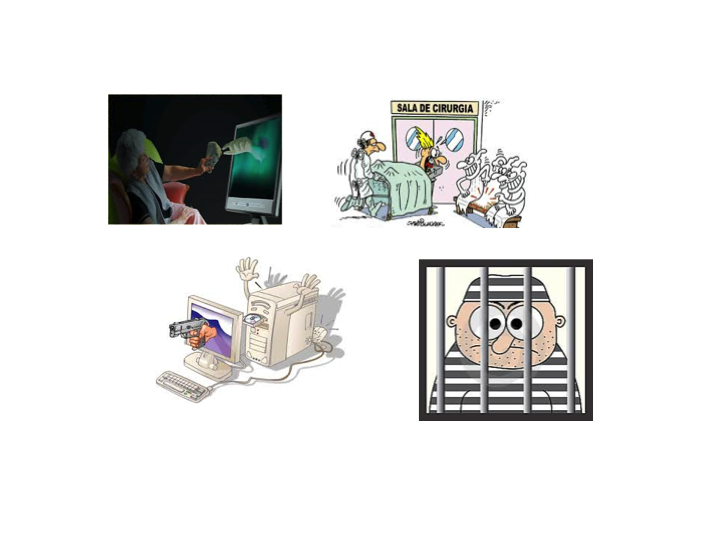
\includegraphics{img/fotos.png}

\end{frame}

\begin{frame}{ROC}

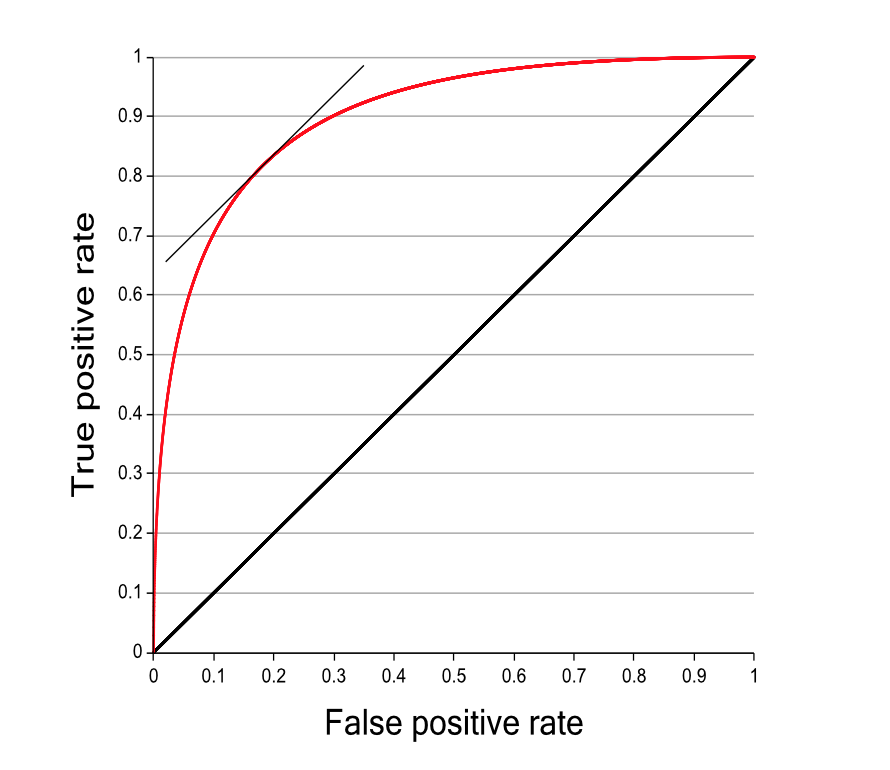
\includegraphics{img/roc.png}

\end{frame}

\begin{frame}{Descipción}

\begin{itemize}
\item
  Attackers have false positives too.

  \begin{itemize}
  \itemsep1pt\parskip0pt\parsep0pt
  \item
    False positive are targets that are attacked but yield nothing.
  \end{itemize}
\item
  False negatives are viable targets that go un-attacked.

  \begin{itemize}
  \itemsep1pt\parskip0pt\parsep0pt
  \item
    Attacks as binary classification decisions.
  \end{itemize}
\end{itemize}

\end{frame}

\begin{frame}{Descipción}

\begin{itemize}
\item
  Attacks are seldom free.

  \begin{itemize}
  \itemsep1pt\parskip0pt\parsep0pt
  \item
    Each potential target represents an investment decision to an
    attacker.
  \end{itemize}
\item
  Victim distribution model.

  \begin{itemize}
  \item
    The attacker does not know with certainty that he will succeed
    unless he tries the attack.
  \item
    Rich does not mean viable.
  \end{itemize}
\end{itemize}

\[ pdf(x|non-viable)=N(0,1)\]

\[pdf(x|viable)=N(\mu,1)\]

\end{frame}

\begin{frame}{Tabla de variables}

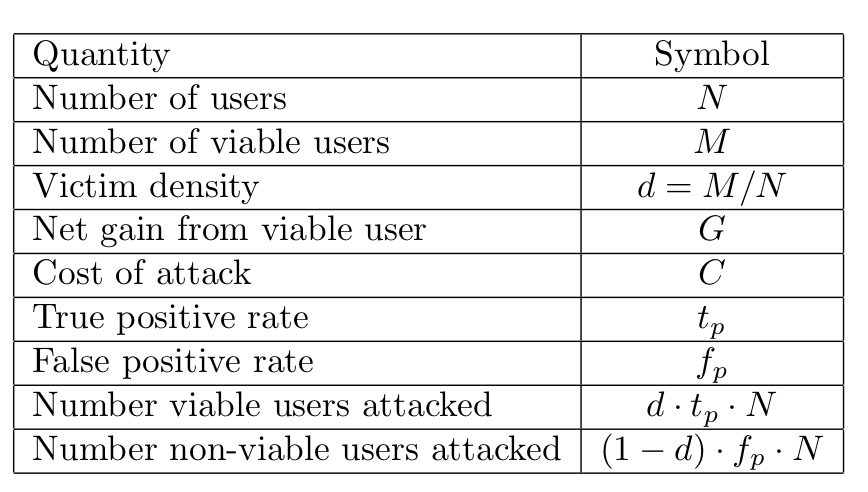
\includegraphics{img/Tabla.png}

\end{frame}

\begin{frame}{Modelo}

\begin{itemize}
\item
  Attack model.

  -Attack if: \[P\{viable|x_i\}*G > P\{non viable|x_i\}*C\]

  -Expected return:
  \[\mathbb{E}[R] = (d  \cdot t_p  \cdot G - (1 - d)  f_p \cdot C)  N\]
\item
  Ability to discriminate between viable and non viable targets.
  \[cdf(x|viable)  \ \mbox{vs.} \ cdf(x|non viable).\]
\item
  Attack everyone, attack at random.

  \begin{itemize}
  \itemsep1pt\parskip0pt\parsep0pt
  \item
    Expected return:
    \[\mathbb{E}[R] = (d \cdot G - (1 - d) \cdot C) \cdot N\]
  \end{itemize}
\end{itemize}

\end{frame}

\begin{frame}{Modelo}

\begin{itemize}
\item
  Optimal Operating Point. \[ \frac{1-d}{d} + \frac{C}{  G}\]
\item
  As slope increases fewer users are attacked.

  \begin{itemize}
  \itemsep1pt\parskip0pt\parsep0pt
  \item
    As slope increases not only are fewer total targets attacked, but
    fewer viable targets are attacked.
  \end{itemize}
\item
  If attacking everyone is not profitable slope must be greater than
  unity. \[ d >\frac{C}{  G + C} \]
\end{itemize}

\end{frame}

\begin{frame}{Distribuciones}

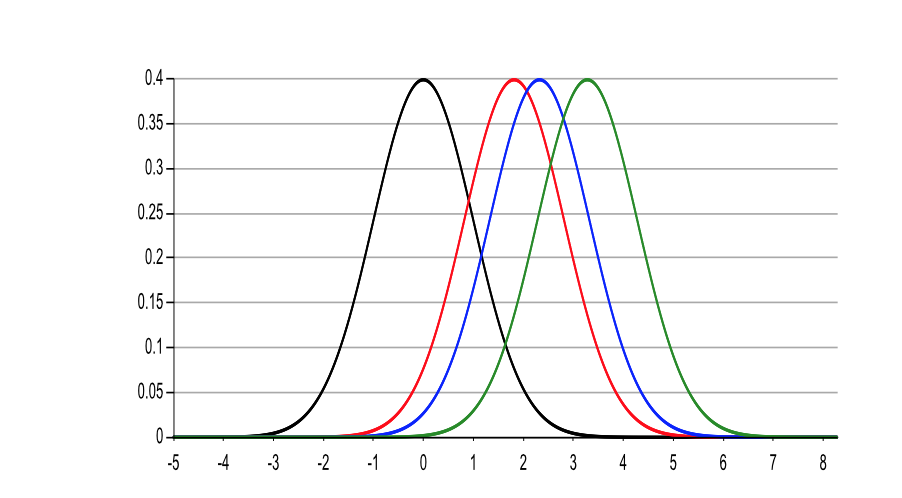
\includegraphics{img/distribuciones.png}

\end{frame}

\begin{frame}{ROC S}

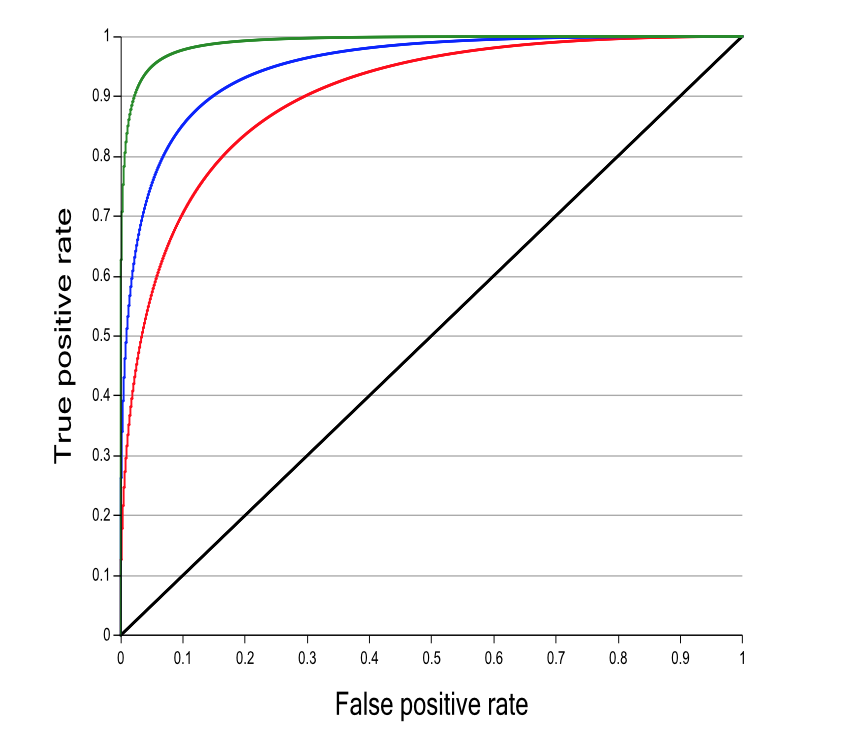
\includegraphics{img/rocs.png}

\end{frame}

\begin{frame}{Pendiente vs $t_p$}

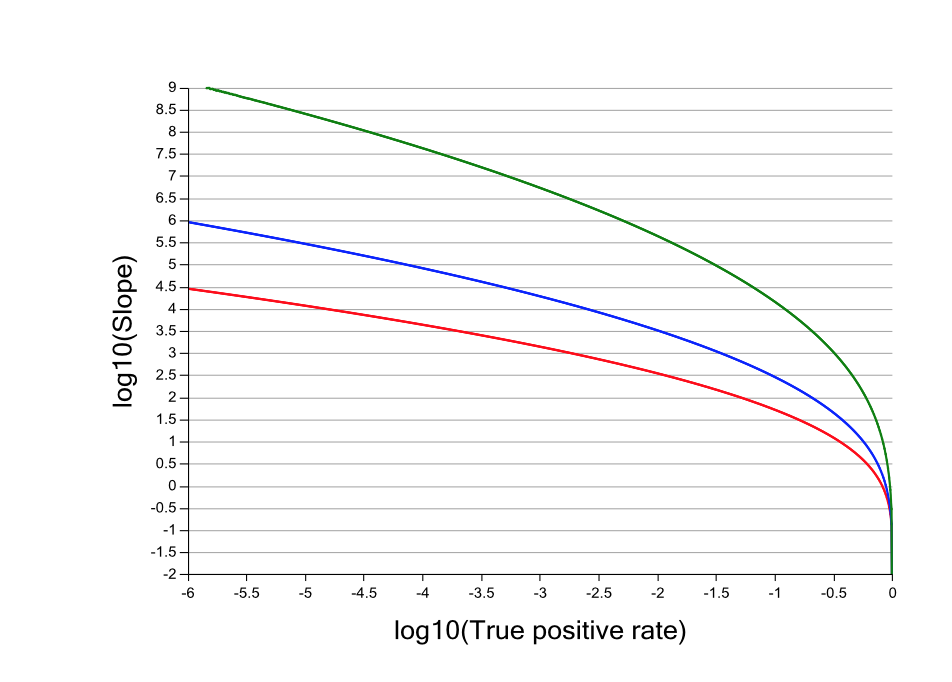
\includegraphics{img/slope.png}

\end{frame}

\begin{frame}{Planteamiento}

\emph{Thus, as slope increases not only are fewer total targets
attacked, but fewer viable targets are attacked.}

\end{frame}

\begin{frame}{Nigerian Scam}

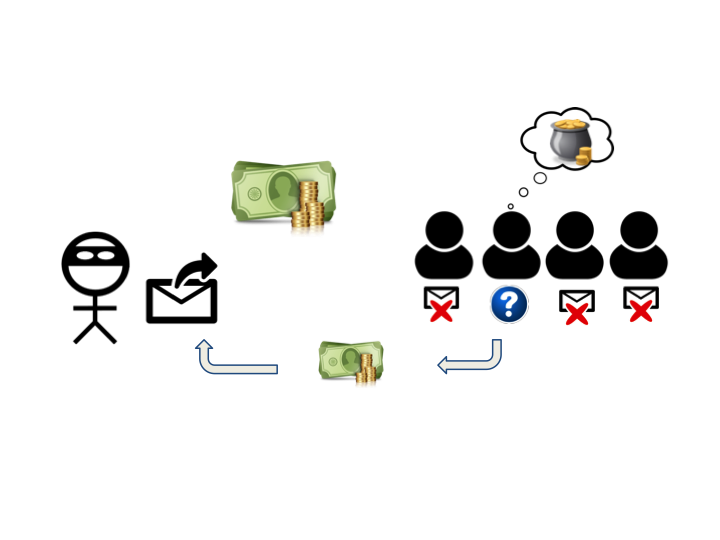
\includegraphics{img/nigeria.png}

\end{frame}

\begin{frame}{¿Por qué los defraudadores dicen que son de Nigeria?}

\begin{itemize}
\itemsep1pt\parskip0pt\parsep0pt
\item
  Quién de ustedes abriría/respondería un correo que tiene en el título
  algo de Nigeria????
\end{itemize}

→ (seguramente nadie!) ¿por qué?

\end{frame}

\begin{frame}{Oportunidades en densidades de víctimas bajas}

\begin{itemize}
\item
  Entrenar un buen clasificador requiere de muchos ejemplos etiquetados.
\item
  Clasificadores con mayor precisión se construyen `fácilmente' en dónde
  menos son requeridos (densidades grandes)
\end{itemize}

\end{frame}

\begin{frame}{¿Cómo funciona?}

\begin{itemize}
\itemsep1pt\parskip0pt\parsep0pt
\item
  El que el correo sea tan obvio para saber que es spam cumple con su
  objetivo: ocupar muy pocos recursos para disminuir el universo de FP y
  enfocarse en los posibles TP → los ingenuos.
\end{itemize}

\end{frame}

\begin{frame}{Utilizar los FP a nuestro favor}

\begin{itemize}
\item
  Responder el correo sabiendo que están buscando víctimas
\item
  Construir modelos que respondan automáticamente a estos correos
\end{itemize}

\end{frame}

\end{document}
